\chapter{Implementation}
	A workflow defined as a graphic summary of the following has been depicted in Figure \ref{work_flow}.

	\section{Dictionary of Songs}
		The trie (Section \ref{sec:trie}) data structure is used to load the Million Song Dataset (Section \ref{sec:million_song_dataset}). Trie not only enables faster searching but also is an ideal data structure for finding the Levenshtein Distances (Section \ref{sec:levenshtein_distance}) on the titles of the songs. The titles of the songs are used as an index for the \emph{trie}. Each node of the \emph{trie} stores with itself some data which is used frequently, for example, its unique track ID using which all other song information can be referenced from the MIllion Song Dataset and artist information. The artist`s name for a song is stored because it along with the title uniquely identifies a song, and is also used for other API calls in the subsequent steps. The \(999,999\) songs (\(1\) song in the dataset was found to be corrupt and hence skipped) from the dataset occupies \(6,510,645\) nodes.
	
	\section{User History}
		A set of \(2614\) users with a considerable amount ($\sim$\(1,000,000\) before cleanup) of playback history has been compiled. These users' histories will serve as the basis for obtaining recommendations from similar users using \emph{collaborative filtering}.
		
		Each track from the users' histories is cross-referenced with those in the million song dataset by searching within the above discussed \emph{trie}. Only those tracks which find a match are kept and the others are discarded; as song information would not be available unless a song is identified. Now, the track names scrobbled by Last.fm are often custom written by third party and/or the users themselves, in which case even a slight change in the name will deem it to be discarded. \emph{Levenshtein Distance} has been used to match each of the fetched song. A threshold distance of \(3\) gives the optimal number of track filtering. Anything lesser would make the filter too strict thus losing too much of valuable user history; whereas keeping it higher will corrupt the data with too many incorrect matches.

		For example, if the title of a song in the history was \emph{``Everything All Of The Time''}, and say, the real name as per the million song dataset was \emph{``'Everything All Of Time'}, with a missing \emph{``The''}. Now, this would require a Levenshtein distance of at least \(3\) for this to be considered; keeping a lower threshold would have lost this track for analysis. Similarly, keeping a higher value of say \(4\), would lead to match some other irrelevant song but with a similar name, like \emph{``Something All Of Time''}. The titles are striped of all special characters and white spaces before matching.
		
		These histories are stored in files on a per user basis. The format is as follows.
		\[ 139940268000 : TRZR!GS128G932C905 \]
		where, the first element is the time, in UTC format, at which the song was listened to; the second element is the \emph{song id} as referenced by the million song dataset to get all other information.
		
		A few other information available with the dataset such as \emph{loudness}, \emph{tempo}, \emph{popularity} are also loaded into memory at this step. This is a part of pre-processing of the data and would considerably lower the runtime of generating the recommendations. These features has been described below in Section \ref{sec:recommend}.
	
	\section{Determine Similar Users}
		A set of \(127\) commonly recognized genres (often referred to as track tags) has been compiled from the \emph{topstags} as recognized by Last.FM. Each song in a user's history is classified in one or more of these genres and a vector is made out of the counts of each of these \(127\) genres. This goes forward to define the user's music preferences.
	
		The similarity between users are determined by their music preferences using the vector of genre counts obtained from each of the songs as described in the previous section. The similarity between user \(X\) and user \(Y\) is calculated on their respective vectors using the \emph{cosine similarity}.
		
		\[ similarity (X, Y) = cos (X, Y) = \frac{A \cdot B}{||A|| ||B||} \]
		
		The top \(k\) similar users have been chosen by sorting on each of their respective similarities with the current user. These users' histories can be searched and used to recommend songs for any given user. 
	
	\section{Recommend Songs}
	\label{sec:recommend}
		\subsection{Defining Mood}
			Assuming an average song has a runtime duration of \(3\) minutes, the mood of a user is determined by the latest \(5\) songs from her history, i.e., $\sim$\(15\) minutes. It is also assumed that the mood of a user changes gradually with time and the songs she listens to is considerably consistant with her mood over this period. A window of consecutive \(5\) songs would hereby define the mood of the user roughly for that period.
			
		\subsection{Collaborative Filtering}
		\label{subsec:collaborative_filtering}
			A mood as per the current user's recent music history is to be searched in the histories of other similar users (by music preferences as determined in the previous step). A rolling window denoting the mood at that particular point in time is compared to that of the fixed current mood again defined by a window of \(5\) songs.
			
			The similarity between any \(2\) windows is determined by the use of the \emph{Hungarian Algorithm} (Section \ref{sec:hungarian}). The cost matrix used by the algorithm is generated by calculating the similarities (Section \ref{subsec:song_similarity}) between each pair of songs, one from each of the \(2\) windows. The algorithm is applied on the thus formed \(5 \times 5\) matrix.
			
			Popularity of each song is a measure on a scale of \(0\) to \(1\). Popularity plays a significant role in the recommendation as users might want to hear new and top of the chart songs even if it does not flare well according to her mood. This information is however stale as of December, 2010.
			
			The song heard right after a given window of \(5\) tracks is presented as a recommendation with a confidence value. This value is a weighted mean of the similarity score between the two windows and the popularity of the song. The weights for similarity and popularity are set to be \(0.8\) and \(0.2\) respectively. This way, each rolling window for each of the similar users are considered, sorted and the top \(5\) recommendations are presented.
			
		\subsection{Song Similarity}
		\label{subsec:song_similarity}
			The following parameters define certain properties of a song and are provided in the million song dataset.
\begin{itemize}
	\item Loudness: It is measured as the logarithm of the maximum power represented by the song. It is measured in decibels (dB). The loudness of a song in the dataset varies in the range of \(-100\) to \(100\). A reference value of -60dB can be used to express the absolute loudness.
	\item Tempo: The average beats per minute of a song contributes to the tempo. This determines the pace of the song, for example, if the song is a slow one or a fast. The tempo of the songs in the dataset varies in the range of \(0\) to \(500\).
	\item Artist: Comparing the artist is crucial, as more often than not, users choose to remain loyal to a certain set of artists. The million song dataset happens to provide a vector of genres for each artist. The vector values are non-negative in nature and denote the count of a set of genres as defined by the dataset. Artist similarity is determined by the use of \emph{cosine similarity} on this vector. A value of \(1\) indicated maximum similarity, whereas, a value of 0, would indicate that the \(2\) artists have nothing in common.
\end{itemize}

			These \(3\) parameters contribute to the determination of the similarity between a pair of songs. A weight of 0.6 has been given to the aritst similarity and a weight of 0.2 each for the normalized absolute difference of both \emph{loudness} and \emph{tempo}.
	
	\section {Recommendation Engine}
		The recommendation system had been developed as a tool. Given a username, whose history is already available with the tool, the tool lists the top \(5\) song recommendations. A user may also modify a few parameters and/or weightages used in the recommendation engine so as to get more custom results. However, a default set of parameters have already been set which in most cases promises to give good results. The tool can be found at \url{http://aritra.cse.iitk.ac.in/amrs/}.
		
		\subsection{Tools/Libraries}
\begin{itemize}
	\item Eclipse: An Integrated Development Environment helped speed up the process of coding and its subsequent debugging.
	\item Java: Being a very common and widely used programming language, loads of  documentation and third party libraries are avialable.
	\item Maven: A dependency resolver fetching all the required dependencies given the name and version of the required libraries.
	\item Jedis (Redis): A java implementation of the Redis DB server. Redis is an in-memory key-value pair DB.
	\item Apache Tomcat: An HTTP servlet implement in and for java execution environments.
\end{itemize}

		\subsection{System Requirements}
		The code and tests have been successfully run on the following configuration. Any system with a configuration equal or higher than this should be able to do the job faster.
\begin{itemize}
	\item RAM: 16GB; fails to run on 8GB, due to the high amount of in memory data.
	\item CPU: Intel Core i7, 4th Generation; have used all 8 virtual cores with hyper-threading, with lower CPU, processes would take longer to complete.
	\item HDD: 280GB dedicated; Million Song Dataset is the only component using considerable persistent memory. Storing user history and codes consume very minimal data storage (in MBs).
	\item Internet Connection \emph{(optional)}: A suitably fast internet connection to getch user history and a few song information. Slower internet speeds might slow down the entire workflow. This is required for pre-processing when all the required data is collected. Alternatively, the whole pre-processed data can be imported by any means.
\end{itemize}
		
		\subsection{Optimizations}
\begin{itemize}
	\item Parallelization: Since, gathering data for every user is fairly independent of each other, these tasks have been implemented in parallel. Also, during the recommendation, once the set of similar users have been collected, suggesting songs per user can again be done in parallel. 16 threads has been found to be the optimal for speed on a CPU with 8 virtual cores (2 hyperthreads per core).
	\item On-Demand: Most songs from the dataset would not be required for recommending, and might consume some valuable runtime. The songs are loaded in the memory at the first missed access. This not only ensures faster runtime but also a lower comsumption of physical memory.
	\item Load Minimal Data Efficiently: Only song data like \emph{loundess}, \emph{tempo} and \emph{popularity} that is required for recommending is loaded into memory. This data is stored in a serialized JSON format. This lightens the overhead of high-level data structures.
	\item Prevent File Access: Each song's information in the million song dataset is stored away in a separate file for each. This heightens the overhead of several files being opened and closed at runtime. Also, there is a limit imposed by the OS to the number of files that can remain open at any given point of time. Thus, only the required information has been extracted, compressed into a serialized format and loaded in memory on an on-demand basis.
\end{itemize}
	
		\subsection{Complications}
\begin{itemize}
	\item Last.FM API: The API is not very robust when multiple calls are made in a short span of time. Several of the calls tend to get failed resulting in the obtained history being corrupted. This restricts the use of multi-threading to fetch user data, which would have improved the runtime significantly.
\end{itemize}
	
		\subsection{Improvements}
\begin{itemize}
	\item Distributed Systems: It gives advantages in terms of more number of CPUs and thus more threads at work, enabling to reduce the runtime considerably. Also, the Last.FM API finds itself in a bit of fix when several calls are being made at the same time from the same computer; this also then can be relieved. This would also enable load balancing the recommendation requests.
	\item NFS: Using an NFS over a local network could shared the dataset and user histories across all the involved machines.
\end{itemize}

	\section{Work Flow Summary}
		\begin{figure}[h!]
			\centering
			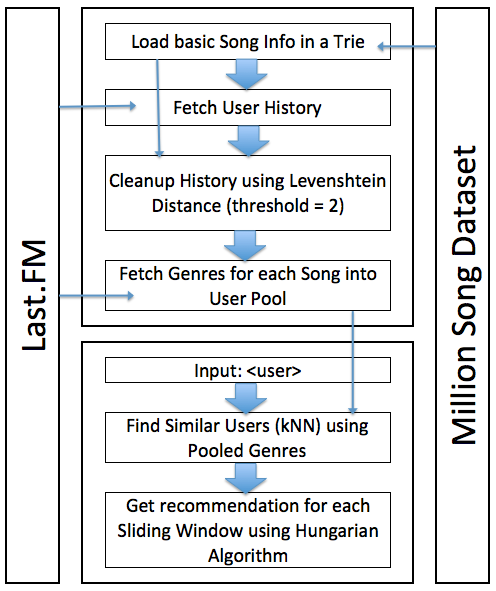
\includegraphics[width=15cm]{work_flow.png}
			\caption{Work Flow\label{work_flow}}
		\end{figure}
			